\chapter{实验}
本章将根据

\section{公平性研究实验}
实验在SUMO(simulation of Urban MObility)\footnote{http://sumo.dlr.de/index.html}仿真平台上进行,利用该模拟器可以方便地实时获取车辆状态,并通过改变交通信号来控制交通运行。我们实现了一个四路交叉口作为我们的实验场景,
交叉口与四个150米长的路段相连,每条道路有三条引入车道和三条引出车道。

我们将N-S方向的道路设置为主干道,车辆到达量更多,将W-E方向的道路设置为次干道,车辆到达量较少。车辆到达服从泊松分布,这里我们设置N-S方向道路的交通流量比率为$\rho$,W-E方向道路的交通流量比率为$1-\rho$,$\rho$值越高,交通流量不平衡的状况越严重。
为了对我们的方法进行综合评价,我们在不同的$\rho$值下进行了实验。注意,为了简化环境,这里我们不考虑行人交通的影响。

\subsection{评价指标}
我们使用以下指标来评估不同方法的效率和公平性表现:
\begin{itemize}
    \item 行驶时间:车辆行驶时间是指车辆进出路口的时间差。现有的大部分工作都集中在最小化所有车辆通过交叉路口的平均行驶时间。
    \item 延误时间:车辆延误时间是车辆通过交叉路口的实际时间与预期时间(以最高限速通过交叉路口所需的时间)之间的差值。
    \item 驾驶体验得分:此外,我们提出了一种新的评价指标,称为驾驶体验得分(Driving Experience Score,DES),来量化驾驶员的满意度,具体评分标准见下表:
        \begin{table}[htb]
            \caption{驾驶体验得分标准}
            \begin{tabular}{cc}
            \toprule
            延误时间(s) & DES \\
            \midrule
            $d \leq 40$ & 5\\
            $40 < d \leq 80$ & 4 \\
            $80 < d \leq 120$ & 3 \\
            $120 < d \leq 160$ & 2 \\
            $d > 160$ & 1 \\ 
            \bottomrule
            \end{tabular}
        \end{table}
        事实上,可能有更多的因素需要考虑(如燃油消耗),但是这里的目的是为了缓解车辆的过度延误情况,因此我们这里用延误时间作为评价标准。
\end{itemize}
\subsection{比较方法}
\begin{itemize}
    \item FT(Fixed-Time Control\cite{miller1963settings}):这种方法以预先设定的方式循环改变信号。
    \item SOTL(Self-Organizing Traffic Light Control\cite{cools2013self}):这是一种根据预先设定的阈值来改变信号的自适应方法。如果等待的车辆数量超过了这个阈值,则切换到下一个信号相位。
    \item LIT\cite{zheng2019diagnosing}:这是一种基于学习的方法,比大多数现有的致力于提高通行效率的方法效果更好。
    \item FIT(\textbf{F}airness-aware \textbf{I}ntelligent \textbf{T}raffic Light Control):我们的方法。
\end{itemize}
\subsection{总体表现}
首先,我们通过实验评估了不同方法的通信效率的表现,为了得到一个综合的结果,我们在不同的$\rho$值下进行了实验,实验结果如\autoref{}所示。
\begin{figure}[htb]
    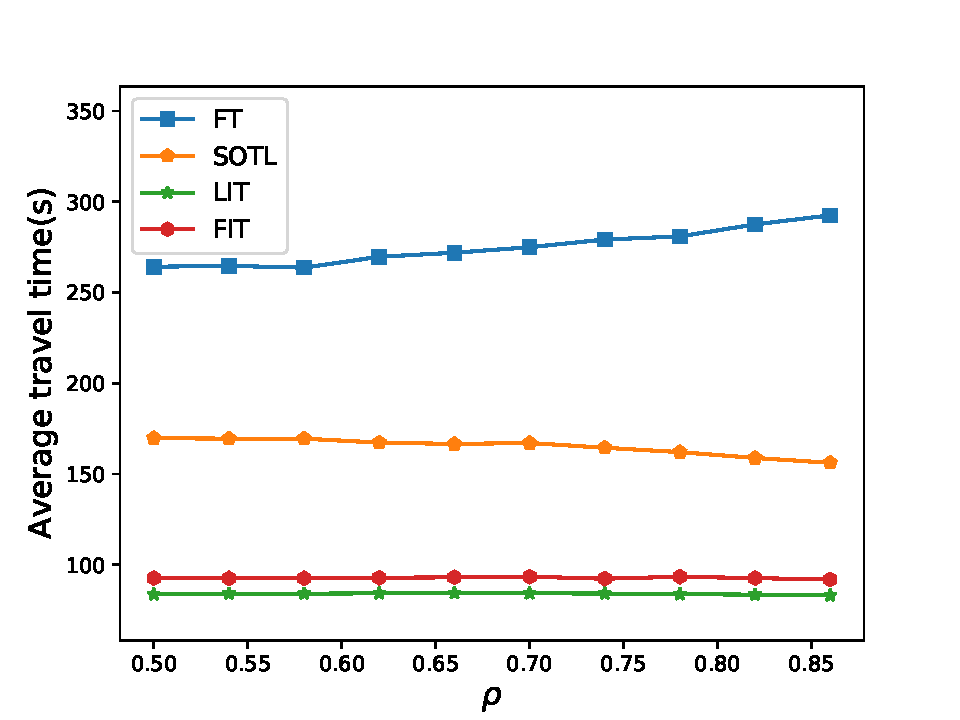
\includegraphics[width=12cm]{fig/efficiency.pdf}
    \caption{效率}
    \label{fig:efficiency}
  \end{figure}

\section{通信研究实验}